\let\negmedspace\undefined
\let\negthickspace\undefined
\documentclass[journal]{IEEEtran}
\usepackage[a5paper, margin=10mm, onecolumn]{geometry}
\usepackage{lmodern} 
\usepackage{tfrupee} 
\setlength{\headheight}{1cm}
\setlength{\headsep}{0mm}   

\usepackage{gvv-book}
\usepackage{gvv}
\usepackage{cite}
\usepackage{amsmath,amssymb,amsfonts,amsthm}
\usepackage{algorithmic}
\usepackage{graphicx}
\usepackage{textcomp}
\usepackage{xcolor}
\usepackage{txfonts}
\usepackage{listings}
\usepackage{enumitem}
\usepackage{mathtools}
\usepackage{gensymb}
\usepackage{comment}
\usepackage[breaklinks=true]{hyperref}
\usepackage{tkz-euclide} 
\usepackage{listings}                             
\def\inputGnumericTable{}                                 
\usepackage[latin1]{inputenc}                                
\usepackage{color}                                            
\usepackage{array}                                            
\usepackage{longtable}                                       
\usepackage{calc}                                             
\usepackage{multirow}                                         
\usepackage{hhline}                                           
\usepackage{ifthen}                                           
\usepackage{lscape}
\usepackage{xparse}

\bibliographystyle{IEEEtran}

\title{4.7.56}
\author{EE25BTECH11059 - Vaishnavi Ramkrishna Anantheertha}

\begin{document}
\maketitle

\renewcommand{\thefigure}{\theenumi}
\renewcommand{\thetable}{\theenumi}

\numberwithin{equation}{enumi}
\numberwithin{figure}{enumi} 

\textbf{Question}:
Find the equation of the line whose perpendicular distance from the origin is $4$ units and the angle which the normal makes with positive direction of x-axis is $15^\circ$

\textbf{Solution 1: }
\begin{table}[H]    
  \centering
  \begin{tabular}{|c|c|}
\hline
\textbf{Name} & \textbf{Value} \\ \hline
$\vec{A}$ & $\myvec{2 & 1 \\0 & 3}$ \\ \hline
\end{tabular}

  \caption{Variables Used}
  \label{tab:4.7.56}
\end{table}

Let eq of line be
\begin{align}
\vec{n^T}\vec{x}=c
\end{align}
where,
\begin{align}
\vec{n}=\myvec{cos 15^\circ
               \\
               sin 15^\circ}
\end{align}
 eq of line is
\begin{align}
\myvec{cos 15^\circ & sin 15^\circ}
\vec{x}
=c\\
\end{align}
As distance from origin (d)=$4$ units
\begin{align}
    \frac{|c|}{\|n\|}=4\\
    \frac{|c|}{1}=4\\
    c=\pm 4
\end{align}   


Hence eq of line is 
\begin{align}
\myvec{cos 15^\circ & sin 15^\circ}
\vec{x}
=\pm4
\end{align}

Refer to Figure

\begin{figure}[H]
\begin{center}
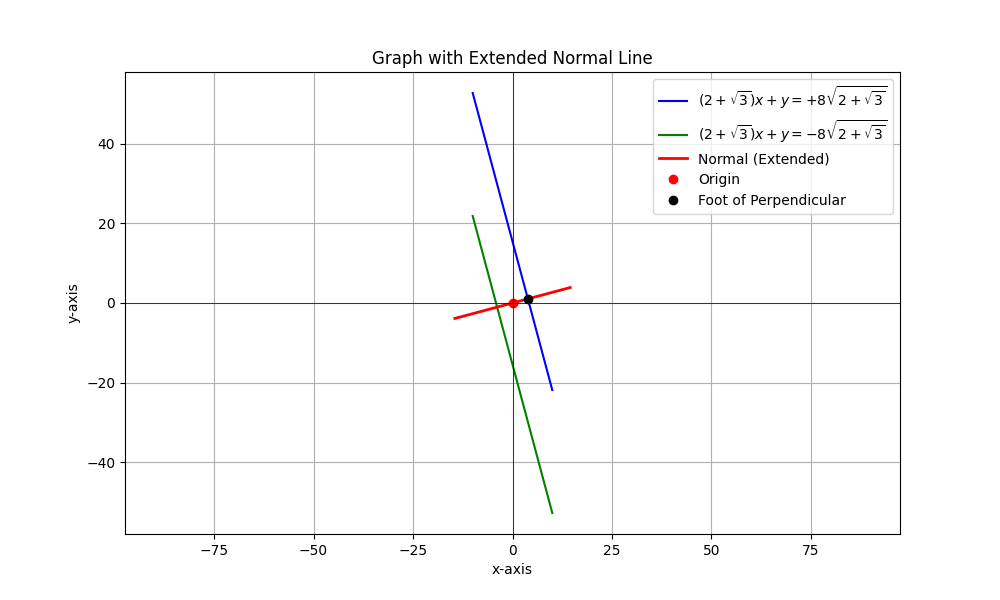
\includegraphics[width=0.6\columnwidth]{figs/graph7.png}
\end{center}
\caption{}
\label{fig:Fig}
\end{figure}
\end{document}